
We experimented with HSLDA for prediction in two domains: predicting medical
diagnosis codes from hospital discharge summaries and predicting product
categories from Amazon.com product descriptions.

%In the section we describe the application of HSLDA for prediction
%in two hierarchically structured domains. Firstly, we describe using
%discharge summaries to predict diagnoses, encoded as ICD-9 codes.
%Discharge summaries are documents that are authored by clinicians
%to summarize the course of a hospitalization. ICD-9 codes are used
%mainly for billing purposes to indicate the conditions for which a
%patient was treated. Secondly, we describe using Amazon.com product
%descriptions to predict product categories.

\subsection{Data and Pre-Processing}

\subsubsection{Discharge Summaries and ICD-9 Codes}

Discharge summaries are authored by clinicians to summarize the course of a
hospitalized patient. The summaries typically contain a record of the patient
complains, findings and diagnoses, along with treatment and hospital course.
For each admission trained medical coders review the information in the
discharge summary and assign a series of diagnoses codes. Coding follows the
ICD-9-CM controlled terminology, an international diagnostic classification for
epidemiological, health management, and clinical
purposes.\footnote{http://www.cdc.gov/nchs/icd/icd9cm.htm} As such, the ICD-9
codes constitute a labeling of a patient's diagnoses based on a discharge
summary. The ICD-9 codes are organized in a rooted-tree structure, with each
edge representing an is-a relationship between parent and child, such that the
parent diagnosis subsumes the child diagnosis. For example, the code for
{}``Pneumonia due to adenovirus'' is a child of the code for {}``Viral
pneumonia,'' where the former is a type of the latter.  It is worth noting that
the coding can be noisy. Human coders sometimes disagree~\cite{Challenge07},
tend to be more specific than sensitive in their
assignments~\cite{Birmetal2005}, and sometimes make
mistakes~\cite{FarzandipourEtAl10}. 

The task of automatic ICD-9 coding has been investigated in the clinical
domain. Much of the work was triggered by the 2007 medical NLP community
challenge~\cite{Challenge07}. The data in the challenge, however, differs from 
ours in its scope. The datasets were smaller (1,000 training and 1,000 testing
documents) and focused on radiology reports with a restricted number of ICD-9
codes (45 of them, compared to 7K+ in our dataset). Methods ranged from manual
rules to online learning~\cite{Crammer2007,Goldstein2007,Farkas2008}.
Other work had leveraged larger datasets and experimented with K-nearest
neighbor, Naive Bayes, support vector machines, Bayesian Ridge Regression, as
well as simple keyword mappings, all with promising
results~\cite{LarkeyCroft95,RibeiroNeto2001,PakhomovEtAl06,Ruch2008,Lita2008}.

Our dataset was gathered from the clinical data warehouse of
NewYork-Presbyterian Hospital. It consists of 6,000 discharge summaries and
their associated ICD-9 codes (7,298 distinct codes overall), representing all
the discharges from the hospital in 2009. Summaries have 8.39 associated ICD-9
codes on average (std dev=5.01) and contain an average of 536.57 terms after
preprocessing (std dev=300.29). We split our dataset into 5,000 discharge
summaries for training and 1,000 for testing.

The text of the discharge summaries was tokenized with
NLTK.\footnote{http://www.nltk.org} Vocabulary was determined as the top 10,000
tokens with highest document frequency (exclusive of names,
places and other identifying numbers). Each discharge summary is thus
represented as counts over the 10,000-word vocabulary. The study was approved
by the Institutional Review Board and follows HIPAA (Health
Insurance Portability and Accountability Act) privacy guidelines.

%For each hospitalization there are usually several ICD-9 codes assigned
%for billing purposes. These codes are known to be quite specific but
%not very sensitive \citep{}. Regardless of that fact,
%this is one of the only sources for information on patient diagnoses
%aside from the free text. %Aside from prediction, one of the goals is to compare the sensitivity of predictions from the HSLDA model in comparison to the codes in a case where a test closer to ground truth is available. For this we will compare whether predictions for the ICD-9 code associated with anemia are better predicted by HSLDA or by the ICD-9 codes. Anemia was chosen because hemoglobin values are readily available and the definition of anemia according the World Health Organization is approximately 12.5, with a threshold of 12 for women and 13 for men [citation].

\subsubsection{Product Descriptions and Categorizations}

Amazon.com, an online retail store, organizes its catalog of 
products in a hierarchy and provides product descriptions
for most products in their catolog.  Products can be discovered by users
through query-based searching or through product category exploration. Top-level
product categories are displayed on the front page of the website and lower
level categories can be discovered by choosing one of the top-level categories.
Products can exist in multiple locations in the hierarchy.

In this experiment, we obtained Amazon.com product categorization data from 
the Stanford Network Analysis Platform (SNAP) dataset~\citep{SNAP}. 
Product descriptions were obtained separately from the
Amazon.com website directly. We limited our dataset to the collection of DVDs
in the product catalog.

We were able to deduce the structure of the
hierarchy for the Amazon.com products because all ancestors in the
hierarchy were included with each category label. For example, {}``DVD / Genres
/ Science Fiction \& Fantasy / Classic Sci-Fi'' is a single product category 
for the DVD, {}``The Time Machine.''

Our dataset contains 15,130 product descriptions for training and 1,000
for testing. The product descriptions are shorter than the discharge summaries
(91.89 terms on average, std dev=53.08). Overall, there are 2,691 unique codes.
Products are assigned on average 9.01 codes (std dev=4.91). The vocabulary
consists of the most frequent 30,000 words omitting stopwords. 

\subsection{Comparison Models}

We evaluated HSLDA along with three other closely related models against 
these two datasets. The comparison models included sLDA with independent 
regressors (hierarchical constraints on labels ignored), HSLDA fit by 
performing LDA followed by tree-conditional regressions, and HSLDA fit 
with fixed random regression parameters. These models were chosen to 
highlight several aspects of the model including performance in the absence 
of hierarchical constraints, the effect of the combined inference procedure, and regression
performance attributable solely to the hierarchical constraints.

sLDA with independent regressors is the most salient comparison model
for our work. The distinguishing factor between HSLDA and sLDA is the
addition structure imposed on the label space, a distinction that we
hypothesize will result in a difference in predictive performance. 
Aside from this, all other features of sLDA are preserved between the two models.

There are two components to HSLDA, LDA and a hierarchically constrained response.
The second comparison model is HSLDA fit by performing LDA first followed by
performing inference over the hierarchically constrained label space. In this
comparison model, the separate inference processes do not allow the responses
to influence the low dimensional structure inferred by LDA. Combined inference
has been shown to improve performance in sLDA \citep{BleiMcAuliffe2008}. This
comparison model examines not the structuring of the label space, but the benefit
of combined inference over both the documents and the label space.

The last comparison model is HSLDA with fixed and randomly selected regression
parameters. There is a baseline benefit that the structure in the label space 
provides for the prediction of labels. This comparison model is intended to
quantify the contribution of the structure alone.

For all of these models, particular attention was payed to the settings of the
prior parameters for the regression coefficients. These parameters implement an
important form of regularization in HSLDA. In the setting where there are no negative
labels, a Gaussian prior over the regression parameters with a negative mean implements
a prior belief that missing labels are likely to be negative. We evaluated model performance 
for all three models with a range of values for $\mu$, the mean prior parameter for regression coefficients
($\mu\in\left\{ -3,-2.8,-2.6,\ldots,1\right\}$).

The number of topics for all
models was set to 50, the prior distributions of
$p\left(\alpha\right)$, $p\left(\alpha^{\prime}\right)$, and $p\left(\gamma\right)$ were gamma distributed with a shape parameter of 1
and a scale parameters of 1000.


\subsection{Evaluation and Results}

%Outline:
%1. Model evaluation goal, metrics
%2. Gold standard(s), properties
%3. Method for prediction w/ details
%4. Discussion of results
%5. Connection of results with contribution and generality etc

We evaluated our model, HSLDA, against the comparison models with a focus
on predictive performance. Predictive performance was measured with
standard metrics - sensitiviy (true positive rate) and 
1-specificity (false positive rate). We evaluate on the two aforementioned
datasets to demonstrate that our model generalizes to two different
domains.

To evaluate the performance of these models, we established a gold standard for comparison.
For each dataset, a held out set of 1000 documents and labels were
reserved for evaluation and predictive performance was evaluated against a standard derived
from the observed labeling. Specifically, ancestors of observed nodes were ignored, observed nodes 
were considered positive and unobserved nodes were considered to be negative. This method of 
defining positive and negative labels was chosen to be as fair as possible to all models
being compared.  In particular, since the sLDA model does not enforce the hierarchical
constraints, the models can be compared on a more equal footing by considering only on the observed labels
as being positive despite the fact that ancestors must also be positive. The gold standard 
defined in this way will likely lead to a slight overestimation of the number of
false positives. It is known that ICD-9 codes lack sensitivity and their use as a
gold standard could lead to correctly positive predictions being labeled as false positives.
However, given that the label space is often large (as in our examples) it is a moderate assumption that
erroneous false positives should not skew results significantly.

Predictive performance in HSLDA is evaluated by $p\left(y_{l,\hat{d}}\mid w_{1:N_{\hat{d}},\hat{d}}, w_{1:N_d,1:D},  y_{l\in\mathcal{L},1:D}\right)$ 
where $\hat{d}$ represents the test document. For efficiency,
the expectation of this probability distribution was estimated in the following way. Expectations
of $\mathbf{\bar{z}}_d$ and $\boldsymbol{\eta}_l$ were estimated with samples from the posterior.
Using these expectations, we performed Gibbs sampling over the hierarchy to acquire predictive
samples for the documents in the test set.

The following are the predictive performance results for the clinical
data given a prior mean for the regression parameters of -1.6. 
The full HSLDA model had a true positive rate of 0.57 
and a false positive rate of 0.13, the sLDA model had a true positive
rate of 0.42 and a false positive rate of 0.07, and the HSLDA model where
LDA and the regressions were fit separately had a true positive rate of 0.39
and a false positive rate of 0.08.

These results indicate that the full HSLDA model predicts more of the the
correct labels at a cost of an increase in the number of false positives
relative to the comparison models.

The following are the predictive performance results for the retail product
data given a prior mean for the regression parameters of -2.2. 
The full HSLDA model had a true positive rate of 0.85 
and a false positive rate of 0.30, the sLDA model had a true positive
rate of 0.78 and a false positive rate of 0.14, and the HSLDA model where
LDA and the regressions were fit separately had a true positive rate of 0.77
and a false positive rate of 0.16. These results follow a similar pattern to the clinical data.

To further explore this tradeoff between the true positive rate and the
false positive rate we evaluated predictive performance for a range of values
for two different parameters - the prior mean for the regression coefficients
and the threshold for the auxiliary variables.  The goal in this analysis
was to evaluate the performance of these models subject to more or less
stringent requirements for predicting positive labels. These two parameters 
have important related functions in the model. The prior mean in combination 
with the auxiliary variable threshold together encode the strength of the prior
belief that unobserved labels are likely to be negative. Effectively, the
prior mean applies negative pressure to the predictions and the auxiliary
variable threshold determines the cutoff.

For each model type, separate models were fit for each value of the 
prior mean of the regression coefficients.  In contrast, to evaluate
predictive performance as a function of the auxiliary variable threshold,
a single model was fit for each model type and prediction was evaluated
based on predictive samples drawn subject to different auxiliary variable
thresholds. These methods are significantly different since the prior mean
is varied prior to inference and the auxiliary variable threshold is varied
following inference.  However, as intended, they both highlight model performance
under more or less stringent requirements for predicting positive labels.

Figure \ref{fig:main_results} shows the predictive performance of HSLDA 
relative to the three comparison models as a function of the prior mean
on regression coefficient. Figure \ref{fig:1a} demo.

\begin{figure}%[htbp]
\begin{center}
%\subfloat[][\label{fig:1a}]{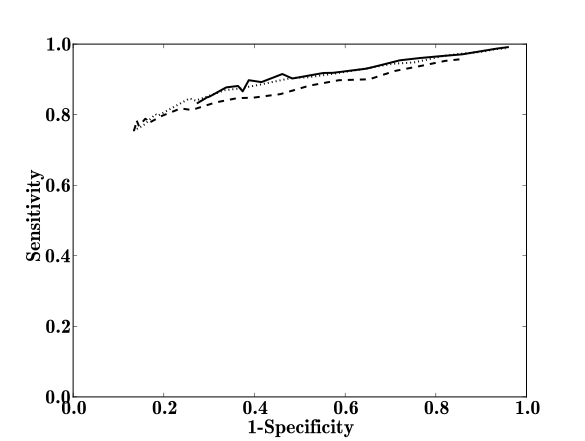
\includegraphics[width=.49\textwidth]{figs/amazon_pred_varying_mu}}
\subfigure[][]{\label{fig:1a}\includegraphics[width=.49\textwidth]{figs/clin_pred_varying_mu}}
%\subfloat[][\label{fig:1c}]{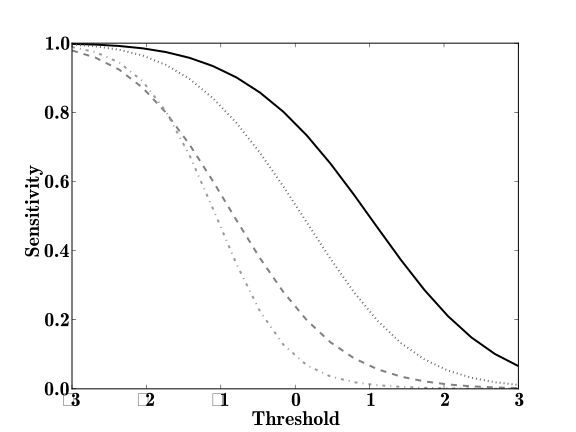
\includegraphics[width=.49\textwidth]{figs/sens_comparison_leafs}}
\subfigure[][]{\label{fig:1b}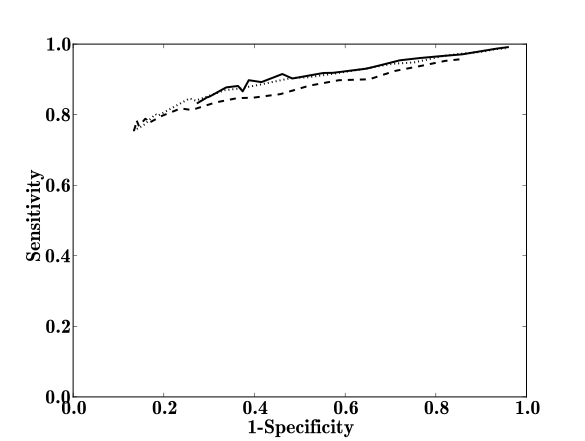
\includegraphics[width=.49\textwidth]{figs/amazon_pred_varying_mu}}
\caption{Out-of-sample ICD-9 code prediction from patient free-text discharge records 
(\subref{fig:1b}). Out-of-sample Amazon product category predictions from 
product free-text descriptions (\subref{fig:1b}). In both figures, solid is 
HSLDA, dashed are independent regressors + sLDA (hierarchical 
constraints on labels ignored), and dotted is HSLDA fit by running LDA first then running 
tree-conditional regressions.}
\label{fig:main_results}
\end{center}
\end{figure}

\begin{figure}[t]
%tbp] %  figure placement: here, top, bottom, or page
 \centering 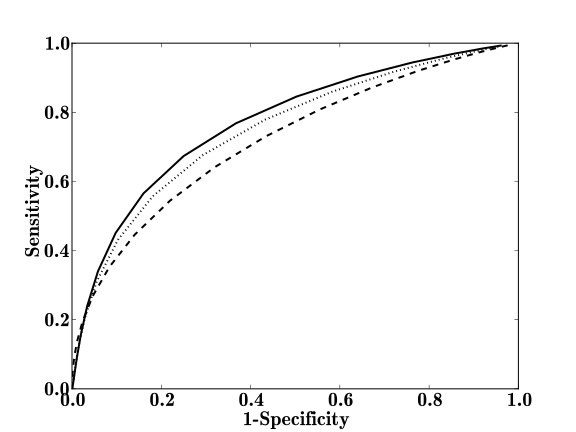
\includegraphics[scale=0.4]{figs/ROC_comparison_leafs} \caption{ROC Curve for clinical data}
\label{fig:clinical_roc} 
\end{figure}
